%! suppress = TooLargeSection
%! suppress = SentenceEndWithCapital
%! suppress = TooLargeSection
% Preamble
\documentclass[11pt]{PyRollDocs}
\usepackage{textcomp}
\usepackage{csquotes}
\usepackage{wasysym}

\addbibresource{refs.bib}
% Document
\begin{document}

    \title{Gripping analysis PyRoll Plugin}
    \author{Christoph Renzing}
    \date{\today}

    \maketitle

    This plugin provides a gripping analysis based on the geometrical conditions inside the roll gap.


    \section{Model approach}\label{sec:model-approach}

    In contrary to flat rolling, the gripping analysis for grooves has to be done locally.
    This is the case, since the roll radius varies and therefore the gripping condition has to be checked locally.
    To archive a local spatial resolution of the roll gap in the x-z plane, the groove and profile are discretized into so called \enquote{Pillar Elements}.
    Since gripping is only possible in areas where the profile is larger than the grooves contour, this discretization is carried out inside the overlapping area.
    This area is defined by the intersection points between groove and incoming profile (see figure~\ref{fig:overlapping-intersection-points}).

    \begin{figure}
        \centering
        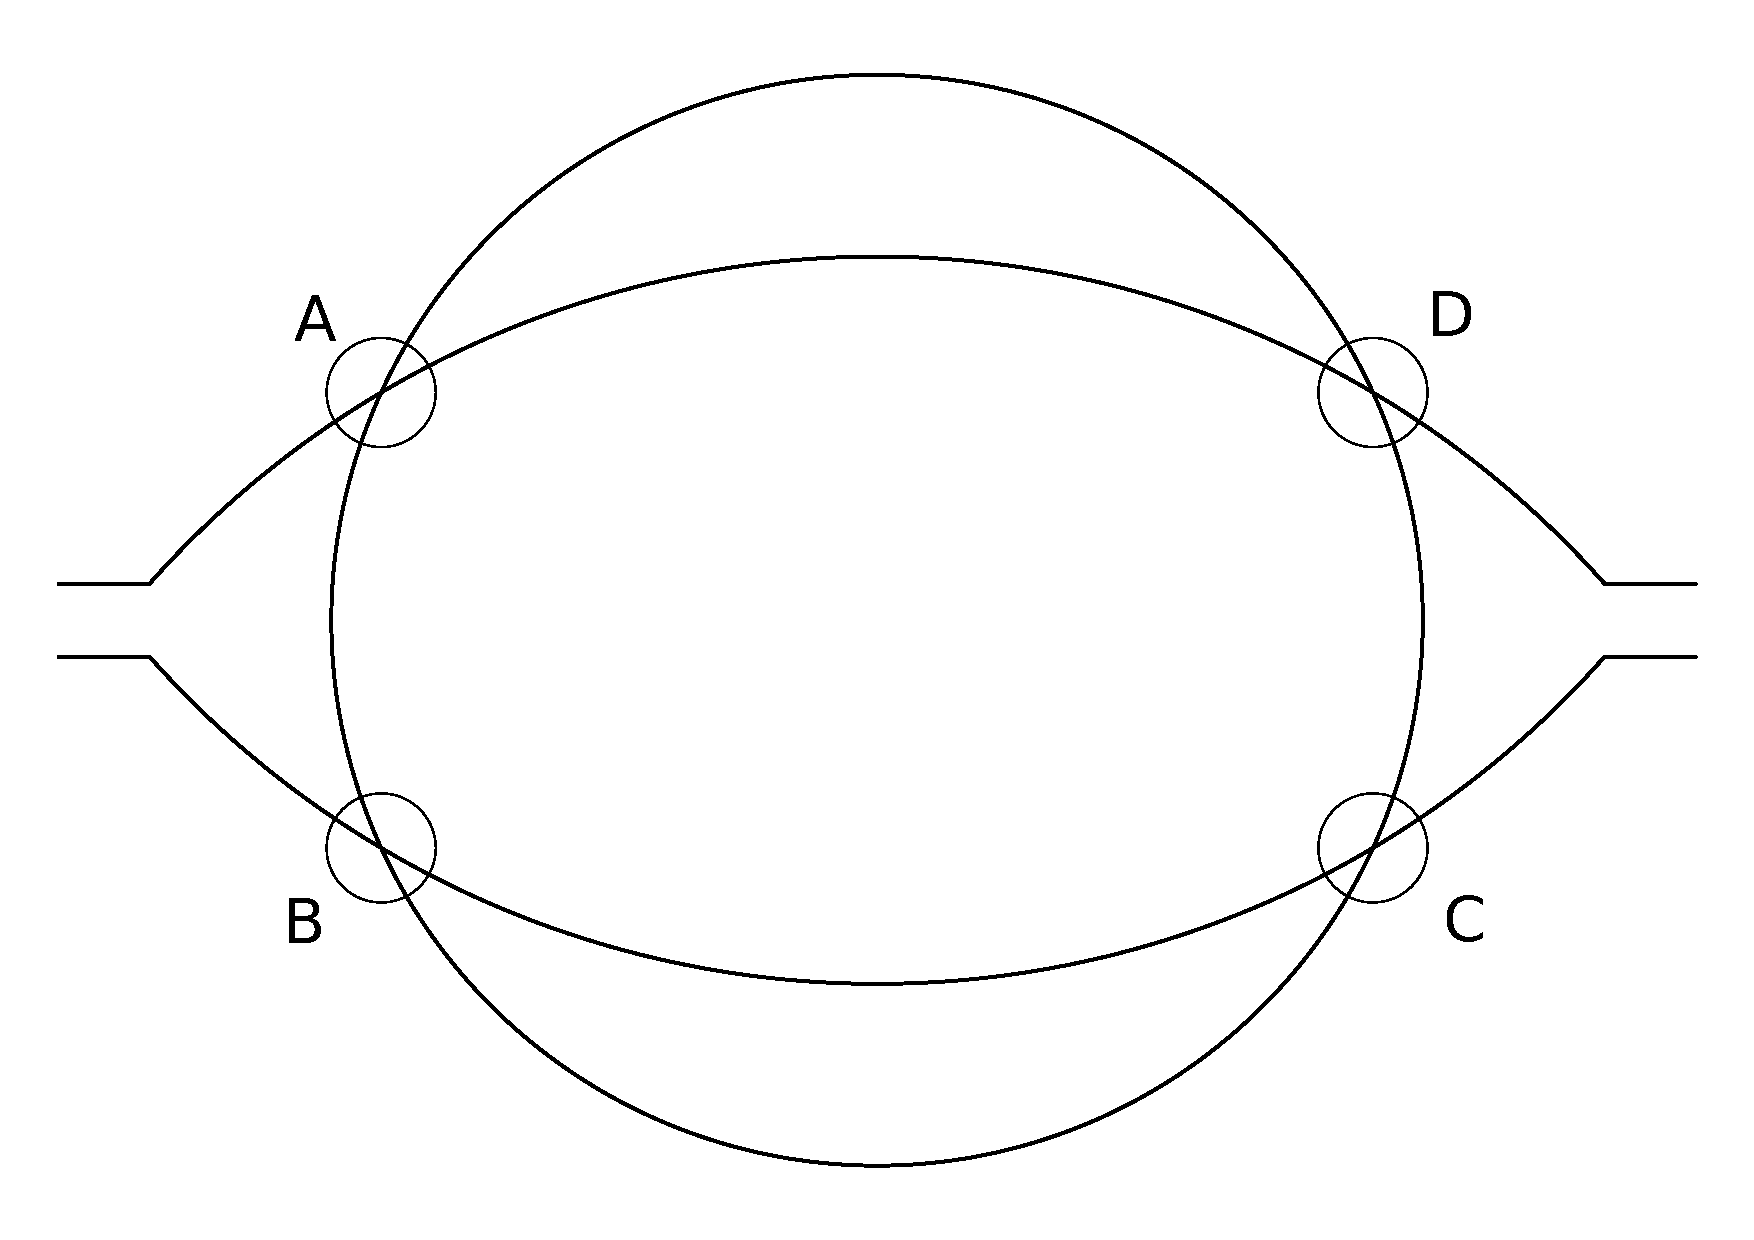
\includegraphics[width=.7\linewidth]{img/intersection_points}
        \caption{Intersection points A to D for a round - oval roll pass}
        \label{fig:overlapping-intersection-points}
    \end{figure}

    \begin{figure}
        \centering
        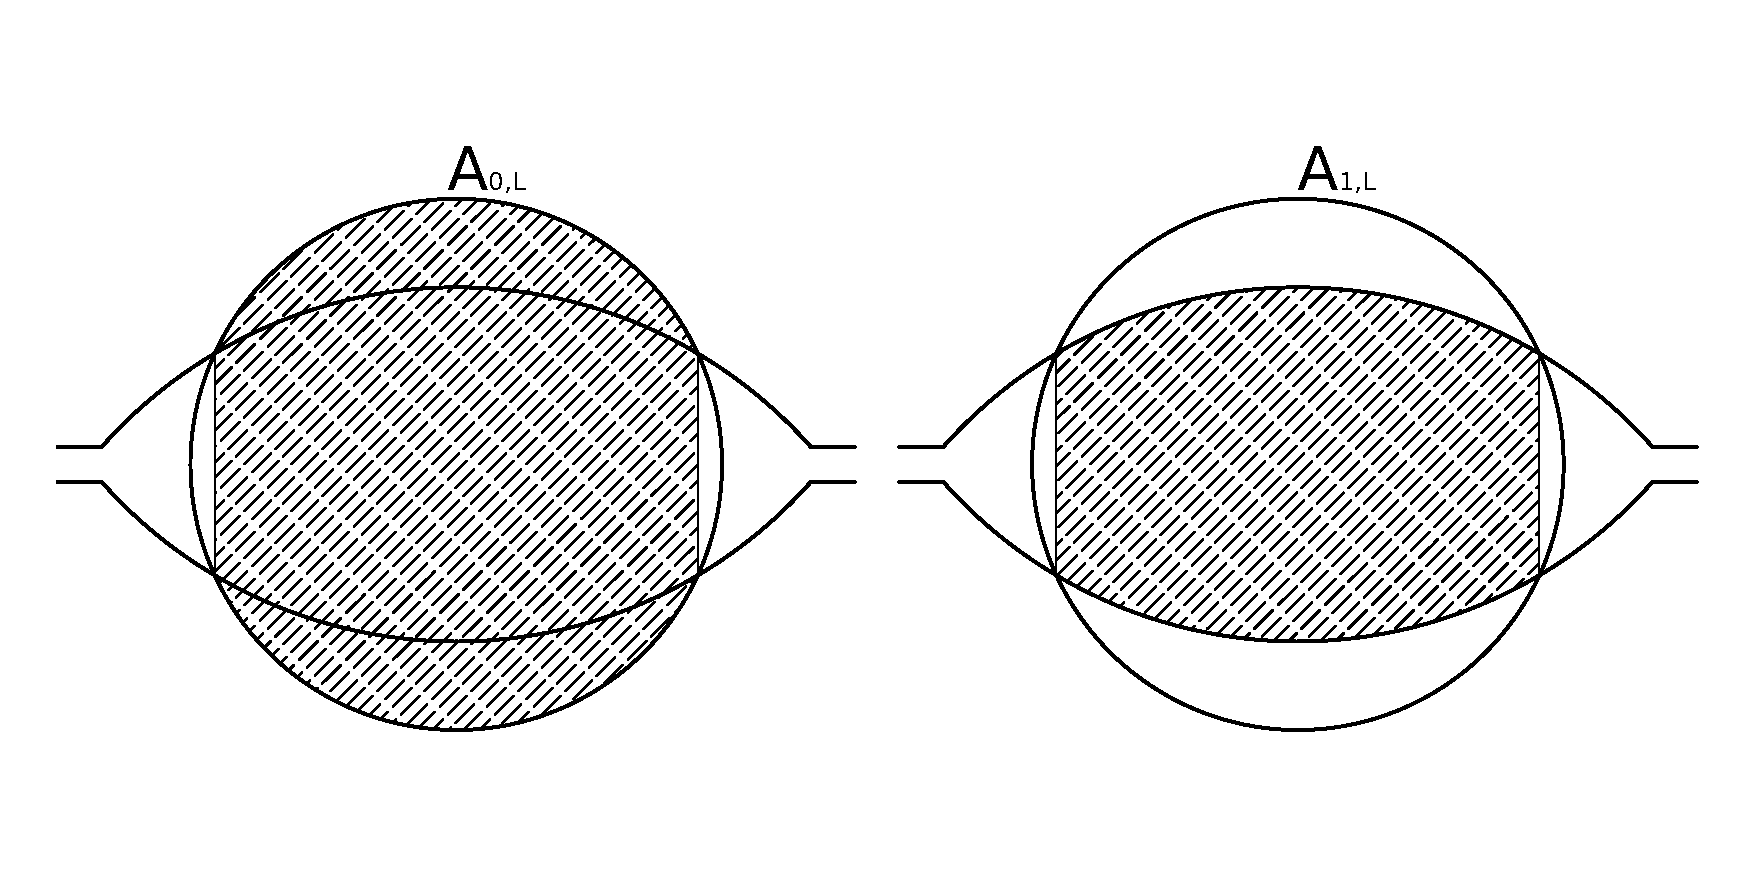
\includegraphics[width=.7\linewidth]{img/overlapping-area}
        \caption{Overlapping area of incoming profile and groove discretized by pillar elements}
        \label{fig:roll-gap-profile-with-pillars}
    \end{figure}

    Using the pilar elements, the local height change is calculated.
    For this, the \listinline{LineString} parts of the upper and lower groove and profile contour which are inside the pillars element boundary are interpolated and
    again discretized into 25 equidistant Points.
    From these points the local reduction is evaluated for the upper and lower part of the pillar (see figure ).
    Using the values, the arithmetic mean value of the reduction for the pilar element is calculated.
    After conducting this evaluation for all pillars, the point for the maximum height reduction in z - direction is searched using numpy.
    The resulting z-coordinate ($z(\Delta h = \Delta h_{\max})$) is used to calculate the local radius of the work roll ($R_{g}$).
    This is done by subtracting the local grooves depth at the position and the nominal roll radius.
    Through this information, the geometric gripping analysis can be evaluated.
    The first assumption for the analysis is that sliding friction,
    represented by Coulombs friction model through a mean friction coefficient $\mu$ is valid for the point of entry of the profile into the roll gap.
    Friction during rolling is necessary to ensure that the rolled material is drawn into the roll gap without external forces.
    These boundary conditions due to friction are called gripping and pull through conditions.
    Figure~\ref{fig:roll-gap-forces} shows the force conditions in the roll gap during gripping.

    \begin{figure}
        \centering
        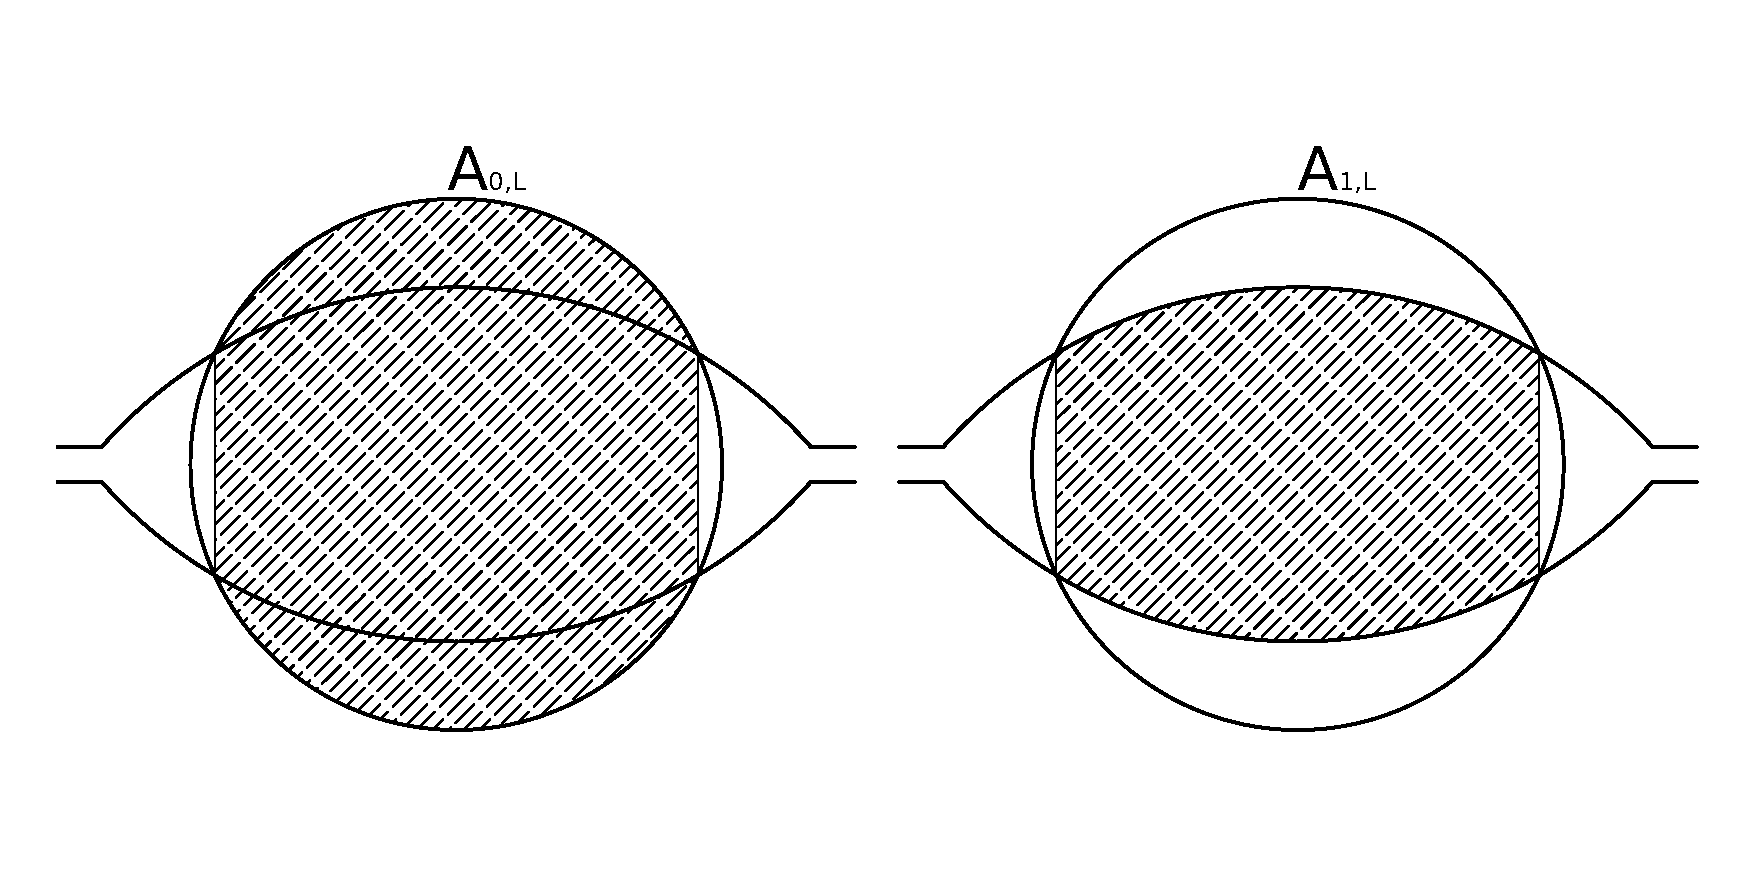
\includegraphics[width=.7\linewidth]{img/overlapping-area}
        \caption{Force acting at the point of gripping in the roll gap}
        \label{fig:roll-gap-forces}
    \end{figure}

    Due to friction, the normal force $F_N$ generates a tangential force $F_T$, see equation~\ref{eq:tangential-force}.

    \begin{equation}
        F_T = \mu \F_N
        \label{eq:tangential-force}
    \end{equation}

    In order for the incoming profile to be drawn into the roll gap, the forces drawing the material into the roll gap ($F_D$),
    must be greater than the ejecting force ($F_E$), so that equation~\ref{eq:forces-while-gripping} applies.

    \begin{equation}
        F_D = \mu F_N \cos\left( \alpha_{g} \right) \geq F_E = \mu F_N \sin\left( \alpha_{g}  \right)
        \label{eq:forces-while-gripping}
    \end{equation}

    From this the grip condition can be determined, see equation~\ref{eq:gripping-condition}.

    \begin{equation}
        \mu \geq \tan\left( \alpha_{g} \right)
        \label{eq:gripping-condition}
    \end{equation}

    The second assumption used for this case, is that the initial contact point between profile and roll happens at a distance which is represented by the contact length.

    \begin{equation}
        L_{d, g} = \sqrt{R_{g} \Delta h_{max} - \frac{\Delta h_{max}^2}{4}}
        \label{eq:contact-length-gripping}
    \end{equation}

    This is valid only for the case, that the material of both the roll and the profile behaves purely plastic.
    Using this assumption, the rolling angle $\alpha$ can be calculated using trigonometric relations.

    \begin{equation}
        \alpha_g = \arcsin\left( \frac{L_{d, g}}{R_{g}} \right)
        \label{eq:gripping-angle}
    \end{equation}

    For calculation of the friction coefficient, the simple model by Ekelund~\cite{Ekelund_1927} is implemented.

    \begin{equation}
        \mu = K_1 K_2 K_3 \left( 1.05 - 0.0005 * \vartheta \right)
        \label{eq:ekelund-friction-coefficient-model}
    \end{equation}


    \section{Usage instructions}\label{sec:usage-instructions}

    The plugin can be loaded under the name \texttt{pyroll\_gripping\_analysis}.
    Besides the hooks \lstinline{gripping-angle}, the implemented \lstinline{number\_of\_pillar\_elements} hook is the entry point for the calculation.
    The calculation is done, using the class \listinline{PillarElement}.
    Several additional hooks on \lstinline{RollPass}, \lstinline{RollPass.Roll} and \lstinline{RollPass.InProfile} are defined, which are used for calculation, as listed in \autoref{tab:hookspecs}.

    \begin{table}
        \centering
        \caption{Hooks specified by this plugin.}
        \label{tab:hookspecs}
        \begin{tabular}{ll}
            \toprule
            Hook name                                       & Meaning                                                                         \\
            \midrule
            \texttt{first\_ekelund\_friction\_coefficient}  & $K_1$ of Ekelunds friction model                                                \\
            \texttt{second\_ekelund\_friction\_coefficient} & $K_2$ of Ekelunds friction model                                                \\
            \texttt{third\_ekelund\_friction\_coefficient}  & $K_3$ of Ekelunds friction model                                                \\
            \texttt{ekelund\_friction\_coefficient}         & $\mu$ resulting from Ekelunds friction model                                    \\
            \texttt{coulomb\_friction\_coefficient}         & Coulombs friction coefficient, defaults to the result of Ekelunds model         \\
            \texttt{upper\_left\_intersection\_point}       & upper left intersection point $A$ in~\ref{fig:overlapping-intersection-points}  \\
            \texttt{upper\_right\_intersection\_point}      & upper right intersection point $B$ in~\ref{fig:overlapping-intersection-points} \\
            \texttt{lower\_left\_intersection\_point}       & lower left intersection point $D$ in~\ref{fig:overlapping-intersection-points}  \\
            \texttt{lower\_right\_intersection\_point}      & lower right intersection point $C$ in~\ref{fig:overlapping-intersection-points} \\
            \texttt{pillar\_elements}                       & List of pillar elements with respected properties                               \\
            \texttt{max\_height\_reduction}                 & List of maximum height reductions                                               \\
            \texttt{point\_of\_max\_height\_reduction}      & List of positions of maximum height reductions                                  \\
            \texttt{gripping\_angle}                        & List of angles resulting of maximum height reductions                           \\
            \texttt{gripping\_evaluation}                   & Result of gripping condition according to equation~\ref{eq:gripping-condition}  \\
            \bottomrule
        \end{tabular}
    \end{table}

    \printbibliography


\end{document}